\documentclass{article}
\usepackage{graphicx} % Required for inserting images
\usepackage{amsmath}
\usepackage{mathtools}
\usepackage{amsfonts} % \mathbb
% \usepackage{centernot}
\usepackage{algpseudocode}
% \usepackage{algorithmicx}
\usepackage{verbatim}

\graphicspath{ {./images/algoritmi-e-strutture-dati/} }

\DeclarePairedDelimiter\ceil{\lceil}{\rceil}
\DeclarePairedDelimiter\floor{\lfloor}{\rfloor}

\title{
	Appunti di Algoritmi e Strutture dati \\
	\large A.A. 2022/2023
}
\date{}

\begin{document}

\maketitle

\section{Fondamenti}

\subsection{Algoritmi e loro rappresentazione}
Un \textbf{problema} é un quesito che richiede la determinazione o la costruzione di uno o piú \underline{enti matematici} che \underline{soddisfino} le \underline{condizioni} specificate nell'enunciato.\\
Con \textit{problema} si denota l'enunciato generale, con \textit{istanza} si denota un caso particolare del problema, ovvero un insieme specifico di dati per il quale si vuole ottenere una soluzione.\\\\
Un \textbf{algoritmo} é una sequenza di azioni \underline{non ambigue} che risolve un problema utilizzando un insieme di azioni elementari, eseguibili da un opportuno esecutore. Con \textbf{programma} si denota la rappresentazione di un algoritmo utilizzando un linguaggio (con opportune "traduzioni") direttamente comprensibile da un elaboratore.\\
L'algoritmo é specificato da un insieme ben definito di dati in input e in output, deve essere eseguibile in un numero finito di passi, fornire il risultato corretto per ogni possibile input ed essere abbastanza generale da essere applicabile a un'intera classe di problemi.\\\\
Lo \textbf{pseudocodice} é un \underline{linguaggio astratto ed informale}, inteso per uso umano, utilizzato per descrivere un algoritmo. Utilizza la struttura di un linguaggio di programmazione normale ma non é vincolato nella sintassi ed é integrabile con linguaggio naturale o notazioni matematiche compatte.

\subsection{Confronto di algoritmi}
Nel confrontare gli algoritmi, ci si astrae da tutti gli aspetti dipendenti dall'implementazione. La risorsa principale su cui ci si basa é il \textbf{tempo di esecuzione}, quantificato non in secondo ma in \underline{accessi alla RAM}.\\
L'algoritmo viene visto come una funzione $f(n)$ (dove $n$ é l'input fornito) di cui si considera solamente il termine dominante (solitamente si trascura anche il coefficiente). Per confrontare due algoritmi, si confrontano le due rispettive funzioni per $n \to \infty$.

\subsubsection{Notazione O-grande}
La crescita asintotica delle funzioni viene descritta con diverse notazioni, la cui maggiormente usata é la notazione $O$ grande (limite asintotico \textbf{superiore}), dove $O$ sta per ordine di grandezza. L'\textbf{ordine di grandezza} é la piú piccola funzione maggiorante (siccome ne esistono infinite).\\\\
Definizione: siano $f : \mathbb{R} \to \mathbb{R}, g : \mathbb{R} \to \mathbb{R}$, $f(x) = O(g(x))$ se $\exists c, x_0 : \forall x > x_0$ si ha $f(x) \le c \cdot g(x)$.\\\\
Esempi
\begin{itemize}
	\item Se si vuole dimostrare $f(x) = x^2+2x+1$ é $O(x^2) \rightarrow x^2+2x+1 \le x^2+2x^2+x^2 = 4x^2 \iff 3x^2-2x-1 \ge 0 \iff x \ge 1$ ($\frac{2 \pm \sqrt{16}}{6} \rightarrow \frac{2 + 4}{6} = 1$). Ho dimostrato che la definizione vale per $n_0=1, c=4$.
	\item Per dimostrare invece che $f(n)=\frac{n(n+1)}{2}$ \underline{non é} $O(n) \rightarrow \frac{1}{2}(n^2+n) \le Cn \iff n^2+n \le 2cn \iff n^2 \le n(2c-1) \iff n \le 2C-1$. Essendo $c$ costante, $\forall c \in R, \exists n \in R : n > 2c-1$, quindi $f(n)$ \underline{non é} $O(n)$.
\end{itemize}
Alcuni ordini di grandezza ben noti in ordine crescente: \textbf{costante} ($O(1)$), \textbf{logaritmico} ($O(\log{n})$), \textbf{lineare} ($O(n)$), \textbf{log lineare} ($O(n \log{n})$), \textbf{polinomiale} ($O(n^k)$ con $k$ costante), \textbf{esponenziale} ($O(c^n)$ con $c$ costante).

\subsubsection{Altre notazioni}
Altre notazioni utilizzate nell'analisi asintotica sono $\Omega$ (Omega grande, limite asintotico \textbf{inferiore}) e $\Theta$ (Theta grande).\\\\
Definizione di $\Omega$: siano $f : \mathbb{R} \to \mathbb{R}, g : \mathbb{R} \to \mathbb{R}, f(n) = \Omega(g(n))$ se $\exists c, n_0 : f(n) \ge c \cdot g(n)$ $\forall n \ge n_0$.\\
É utilizzata nei limiti inferiori di complessitá e per l'analisi del tempo di esecuzione nel caso ottimo.\\\\
Definizione di $\Theta$: siano $f : \mathbb{R} \to \mathbb{R}, g : \mathbb{R} \to \mathbb{R}, f(n) = \Theta(g(n))$ se $\exists c_1, c_2, n_0 : c_1 \cdot g(n) \le f(n) \le c_2 \cdot g(n)$ $\forall n \ge n_0$. Da notare che $f(n) = \Theta(g(n)) \iff f(n) = O(g(n)) \wedge \Omega(g(n))$.\\
$O(fn))$ é spesso usato erroneamente al posto di $\Theta(f(n))$.\\\\
Esistono degli analoghi di $O$ e $\Omega$ che sono $o$ ($o$ piccolo) e $\omega$ (omega piccolo), dove al posto della disuguaglianza ($\le$) si ha la disuguaglianza stretta ($<$).\\\\
Equivalentemente:
\begin{itemize}
	\item[] se $\displaystyle \lim_{n \to \infty} \frac{f(n)}{g(n)} \to c$, allora $f(n) = \Theta(g(n))$
	\item[] se $\displaystyle \lim_{n \to \infty} \frac{f(n)}{g(n)} \to 0$, allora $f(n) = o(g(n))$
	\item[] se $\displaystyle \lim_{n \to \infty} \frac{f(n)}{g(n)} \to \infty$, allora $f(n) = \omega(g(n))$
\end{itemize}

\subsubsection{Caso ottimo, medio, pessimo}
Nell'analisi degli algoritmi si possono analizzare 3 casi: caso ottimo (migliore possibile), medio e pessimo (peggiore possibile). Principalmente si analizza il caso pessimo e il caso medio, anche se l'analisi di quest'ultimo é spesso molto piú complicata delle altre due perché richiede un'analisi statistica.\\\\
Esempio: Ricerca sequenziale.\\
Problema: dato un array $v$ e un valore $x$, restituire l'indice della prima occorrenza di $x$ in $v$, o -1 se $x$ non é presente.\\
\begin{enumerate}
	\item Caso ottimo: l'elemento é all'inizio della lista ($O(1)$)
	\item Caso pessimo: l'elemento é in fondo o non é presente, quindi si itera su tutti gli elementi ($O(n)$)
	\item Caso medio: per ipotesi, l'elemento é sempre presente e la probabilitá $p_i$ che l'elemento si trovi alla posizione $i$ sia la stessa per ogni $i$, quindi $p_i = \frac{1}{n}$. Se l'elemento é nella prima posizione, devo controllare una sola volta, nella seconda due volte, nella terza tre volte e cosí via fino a $n$: questo lo posso esprimere con la somma dei primi $n$ numeri, ovvero con la serie geometrica $\displaystyle \sum_{i=1}^{n} i = \frac{n(n+1)}{2}$. Moltiplico il tutto per la probabilitá $p_i$, che é la stessa per ogni elemento e ottengo $\displaystyle \frac{1}{n} \cdot \frac{n(n+1)}{2} = \frac{1}{2}(n+1)$, ovvero $O(n)$.
\end{enumerate}

\section{Analisi asintotica}
Un algoritmo $A$ ha \textbf{costo di esecuzione} $O(f(n))$ rispetto ad una risorsa di calcolo, su instanze di ingresso di dimensione $n$ se la quantitá $r(n)$ di risorsa sufficiente per eseguire A su una \textbf{qualunque istanza di dimensione} $n$ verifica la relazione $r(n) = O(f(n))$.\\\\
Dato lo pseudocodice, é possibile ottenere il costo di esecuzione analizzando la sua struttura. Ad esempio, data una serie di istruzioni, $t(\mbox{istruzione }1) + \dots + t(\mbox{istruzione }n)$, negli if-else $max(t(\mbox{ sequenza }1), t(\mbox{ sequenza }2))$, nei for e nei while bisogna vedere se il ciclo viene eseguito un numero di volte funzione di $n$ o meno.

\subsection{Algoritmi ricorsivi}
Negli algoritmi ricorsivi, il tempo di esecuzione dell'algoritmo puó essere descritto come la somma dei tempi di esecuzione di $f(n_1), \dots , f(n_k)$ con $n_i < n$, ovvero richiede di calcolare tutti i termini precedenti, fino al caso base.

\subsubsection{Ricerca binaria}
La ricerca binaria ha classe di complessitá $O(logn)$.\\
Il tempo di esecuzione puú essere espresso come:
\begin{equation}
	\begin{cases}
		c_1 \mbox{ se } n = 1 \mbox{ (caso base)} \\
		T(\floor{\frac{n}{2} }) 
		+ c_2 \mbox{ se } n > 1
	\end{cases}
\end{equation}
É dimostrabile con diversi metodi, tra cui:
\begin{enumerate}
	\item Metodo iterativo. Partendo da $\displaystyle T(n)$, devo arrivare al caso base $T(1) = T(\frac{n}{n}$) dimezzando $n$ ad ogni passo. $T(n) = T(\frac{n}{2}) + c_2 = T(\frac{n}{4}) + 2c_2 = T(\frac{n}{8}) + 3c_2 = \dots$\\
	Mi fermo quando $n = 2^k$, quindi dopo $k = log_2{n}$ chiamate ricorsive, per un totale di $ck$ chiamate ($c = c_1 + kc_2$). Quindi, $$T(n) = c \cdot log_2{n} = O(logn)$$
	\item Dimostrazione per induzione. Prima di dimostrare, si "indovina" (grazie anche all'esperienza) la soluzione: $T(n) \le c \cdot log_2{n} (T(n) = O(logn))$.\\
	Assumendo $T(n') \le c \cdot log_2{n'}$  $\forall n > n'$ (\textbf{ipotesi induttiva}), voglio dimostrare che $T(n) \le c \cdot log_2{n}$.\\\\
	$\displaystyle T(n) = T(\frac{n}{2}) + 1 \mbox{ (costante qualsiasi)} \le c \cdot log_2(\frac{n}{2}) + 1 \mbox{ (ipotesi induttiva (} \frac{n}{2} \mbox{ é n'))} \\
	= c \cdot log_2{n} - c \cdot log_2{2} \mbox{ (proprietá del logaritmo) } + 1 \\
	= c \cdot log_2{n} - c \cdot 1 + 1$.\\
	Se $c \ge 1$, allora $$c \cdot log_2{n} + c - 1 \le c \cdot log_2{n} \rightarrow T(n) \le c \cdot log_2{n}$$
\end{enumerate}

\section{Grafi}
Un grafo $G = (V,E)$ é composto da un insieme di \textbf{vertici} $V$ e un insieme di \textbf{archi} $E \subset V \times V$ (non $\subseteq$ perché non si ha un arco tra un vertice e se stesso) che connettono i vertici.

\subsection{Terminologia}

\subsubsection{Grafo orientato/non orientato}
In un grafo \textbf{non orientato}, due vertici $u,v$ sono \textbf{adiacenti} se $\{u,v\} \in E$.\\
In un grafo \textbf{orientato}, se $(u,v) \in E \rightarrow v$ adiacente a $u$ e $(u,v)$ é \textbf{incidente} in $v$.

\subsubsection{Grado, cammino e ciclo}
Il \textbf{grado} di un vertice é il numero di vertici adiacenti ad esso.\\
Il \textbf{cammino} é una sequenza di vertici $v_1, \dots, v_n$ tale che per ogni coppia di vertici consecutivi $v_i, v_{i+1}$, $v_{i+1}$ é adiacente a $v_i$. Un cammino é detto \textbf{elementare} se non ci sono vertici ripetuti. Un \textbf{ciclo} é un cammino elementare in cui il primo vertice coincide con l'ultimo (torna all'inizio).

\subsubsection{Grafo connesso, sottografo}
É detto \textbf{grafo connesso} qualsiasi coppia di vertici unita da almeno un cammino.\\
Un \textbf{sottografo} é un sottoinsieme di vertici e archi di un grafo dato. Una \textbf{componente connessa} é un sottografo connesso massimale.

\subsubsection{Grafo completo}
Un grafo é detto \textbf{completo} se ogni coppia di vertici é connessa da un arco. In questo caso, il numero di archi $m = \sum_{i=1}^{n-1}i = \frac{n(n-1)}{2}$ (ogni nodo é connesso a $n-1$ nodi ($n(n-1)$); infine divido per 2 siccome altrimenti sto considerando gli stessi archi 2 volte).

\subsubsection{Grafo trasposto}
Un grafo é $G^T = (V,E^T)$ é il \textbf{trasposto} di $G = (V,E)$ se $E^T = \{(u,v):(v,u) \in E\}$ (inverte il verso di percorrenza degli archi di $G$).

\subsubsection{Grafo pesato}
In un grafo pesato, agli archi viene associato un valore, detto \textbf{peso} (es. costo necessario per percorrerlo). Il peso é determinato da $p : V \times V \to \mathbb{R}$. Se non specificato, si assume il costo infinito.

\subsection{Alberi}
Un albero é un \textbf{grafo aciclico} (non é possibile compiere un ciclo al suo interno) con un numero di nodi uguale al numero di archi + 1. Puó esistere un nodo particolare chiamato \textbf{radice}, a partire dal quale é possibile raggiungere qualsiasi altro nodo.\\\\
A partire dalla radice, viene definita una \textit{relazione di ordinamento} fra i nodi, basata sulla distanza dalla radice, in cui ogni nodo puó avere un padre e dei figli. Inoltre, é detto \textbf{foglia} un nodo senza successori, mentre se presenta successori é detto \textbf{nodo interno}.\\
Si definisce \textbf{profonditá} di un nodo la lunghezza del cammino dalla radice al nodo, \textbf{altezza} di un nodo la massima lunghezza di un cammino dal nodo a una foglia discendente dal nodo stesso, altezza dell'albero l'altezza della radice (massima lunghezza del cammino che collega la radice a qualsiasi nodo).\\
Un \textbf{livello}/strato consiste di nodi con la stessa profonditá. Il numero di livelli é dato dall'altezza + 1 (radice).\\\\
La rappresentazione grafica di un albero é detta \textbf{arborescenza}.

\section{Ordinamento}
Input: sequenza di $n$ numeri $a_1, a_2, \dots, a_n$\\
Output: i numeri ricevuti in input in ordine crescente: $a_{\pi(1)}, a_{\pi(2)}, \dots, a_{\pi(n)}$, dove $\pi$ é una permutazione degli indici.\\\\
Esempio:\\
$a = [7, 32, 88, 21, 92, -4]$\\
$\pi = [6,1,4,2,3,5]$ (1-based)\\
$a[\pi[]] = [-4,7,21,32,88,92]$\\\\
Piú in generale, dato un array di $n$ elementi, ogni elemento é composto da una \textbf{chiave} (confrontabili tra loro) e un \textbf{valore}. Si vuole permutare l'array delle chiavi in modo che appaiano nell'ordine desiderato.

\subsection{Definizioni}
\begin{itemize}
	\item ordinamento \textbf{in place}: l'algoritmo permuta gli elementi dell'array senza utilizzare un array di appoggio
	\item ordinameno \textbf{stabile}: l'algoritmo preserva l'ordine in cui gli elementi con la stessa chiave appaiono nell'array originale
\end{itemize}

\subsection{Teorema del lower-bound per algoritmi comparison-sort}
Qualsiasi algoritmo comparison-sort (basato su confronti di coppie di elementi) effettua, nel caso pessimo, $\Omega(n \cdot logn)$ (non puó fare meglio di così) confronti per ordinare una sequenza di $n$ numeri.\\\\

\subsubsection{Dimostrazione}
Alla base c'é l'idea che, dato un array di $n$ numeri, esistono $n!$ permutazioni, quindi $n!$ possibili ordinamenti, e ad ogni confronto si dimezzano le possibilitá rimaste.\\
Il caso pessimo é dato dall'altezza dell'albero decisionale associato a questo algoritmo. Siccome l'albero decisionale in questo caso é un \textbf{albero binario} (albero in cui ogni nodo ha al massimo 2 figli), date $n!$ foglie, ha un'altezza $\Omega(nlogn)$, quindi nel caso pessimo vengono eseguiti $\Omega(nlogn)$ confronti.\\\\
Dimostrazioni
\begin{enumerate}
	\item Siccome un albero binario alto $h$ ha massimo $2^h$ foglie, bisogna ottenere $\displaystyle 2^h \ge n!$. Usando la formula di Stirling: $n! > (\frac{n}{e})^n$ $\implies$ $$h \ge log{(\frac{n}{e})^n} = nlog(\frac{n}{e}) = nlogn -nloge = \Omega(nlogn)$$\\
	Si noti che il passaggio da $log_2$ a $log_e$ é semplicemente dato dalla moltiplicazione per una costante
	\item Bisogna ottenere $2^h \ge n! \implies h \ge log(n!)$. Siccome ho $\ge$, se sostituisco a $log(n!)$ qualcosa di piú piccolo, la disuguaglianza resta sempre vera, quindi: $$\displaystyle log(n!) = log(1 \cdot 2 \cdot \dots \cdot \frac{n}{2} \cdot (\frac{n}{2}+1) \cdot \dots \cdot n) \ge log(1 \cdot 1 \cdot \dots \cdot \frac{n}{2} \cdot \dots \cdot \frac{n}{2}) = log(\frac{n}{2})^{\frac{n}{2}} = \frac{n}{2}log(\frac{n}{2}) = \Omega(nlogn)$$\\
	(sostituisco tutti i termini da 1 a $\frac{n}{2}$ con 1 e da $\frac{n}{2}$ a $n$ con $\frac{n}{2}$).
\end{enumerate}

\subsection{Insertion sort}
In questo algoritmo, si parte disponendo gli elementi ordinati nella parte sinistra dell'array, si prende un elemento dalla parte non ordinata e lo si inserisce in maniera ordinata.

\subsubsection{Pseudocodice}
\begin{algorithmic}
\For{$j = 2$ to size($A$)}
	\State $key \gets A[j]$
	\State $i \gets j - 1$	
	\While{$i > 0$ and $A[i] > key$} \Comment{fino a quando il numero é piú grande}
 		\State $A[i+1] \gets A[i]$ \Comment{shifto a destra di 1}
		\State $i \gets i - 1$
	\EndWhile
	\State $A[i+1] \gets key$
\EndFor
\end{algorithmic}

\subsection{Merge sort}
Il merge sort é un algoritmo di ordinamento che si basa sul metodo \textbf{divide et impera}, che consiste nel dividere un problema in sottoproblemi, risolverli e combinare le soluzioni dei sottoproblemi per ottenere la soluzione del problema complesso.\\\\
Dato un vettore $S$, l'algoritmo consiste nel:
\begin{enumerate}
	\item dividere $S$ nei vettori $S_1$ e $S_2$, ognuno con la metá degli elementi di $S$ fino a quando $S$ ha almeno 2 elementi
	\item ordinare gli elementi in $S_1$ e $S_2$ (merge)
	\item mettere insieme gli elementi di $S_1$ e $S_2$
\end{enumerate}
Si parte ordinando 2 vettori da 1 elemento, poi 2 vettori da 2 elementi e cosí via fino ad ordinare i due sottovettori iniziali $S_1$ e $S_2$.\\\\
Il merge é la parte che si occupa di ordinare i sottovettori. Ad ogni ordinamento di 2 vettori di $n$ e $m$ elementi, alloca un vettore di $n+m$ elementi (non in-place). L'ordinamento viene fatto inserendo ogni volta nel vettore allocato il minore degli \textbf{affioranti} (elementi piú a sinistra di ogni vettore, ovvero i piú piccoli).

\subsubsection{Pseudocodice}
Versione ricorsiva non in-place:
\begin{algorithmic}
\Function{mergeSort}{A,p,r}
\If{$p < r$}
	\State $q \gets (p+r)/2$
	\State \Call{mergeSort}{A,p,q} \Comment{ordino la metá di sinistra}
	\State \Call{mergeSort}{A,q+1,r} \Comment{ordino la metá di destra}
	\State \Call{merge}{A,p,q,r}
\EndIf
\EndFunction
\end{algorithmic}

\subsubsection{Esempio}
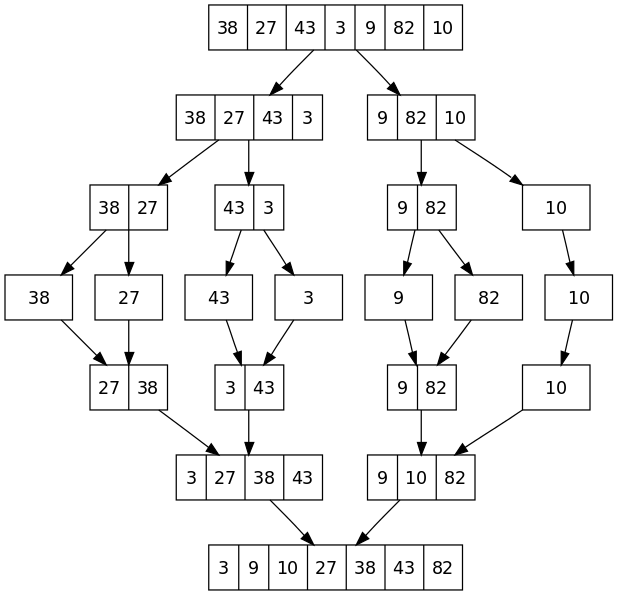
\includegraphics[scale=0.4]{merge-sort.png}

\subsubsection{Complessitá}
La complessitá del merge sort non dipende dalla configurazione iniziale. L'algoritmo fa lo stesso procedimento ogni volta, quindi non esiste un caso pessimo, medio o ottimo:\\
$$T(n) = 2T(\frac{n}{2}) + \Theta(n) = \Theta(nlogn)$$

\subsection{Quick sort}
Il quick sort é un altro algoritmo di ordinamento sempre basato sulla tecnica divide et impera.\\
Consiste nel dividere l'array in 2 parti non vuote basandosi su un elemento detto \textbf{pivot} (selezionato arbitrariamente (es. il primo) o casualmente (minimizza le possibilitá di avere il caso pessimo)), spostando tutti gli elementi piú piccoli del pivot a sinistra e quelli piú grandi a destra. Il procedimento viene iterato fino a quando tutti i gruppi non sono ordinati.\\\\
Il lavoro principale é svolto dalla funzione che si occupa di partizionare:
\begin{itemize}
	\item partendo dall'inizio del vettore, ci si sposta verso il fondo (destra) fino a quando non si trova un elemento piú grande ($\ge o >$ arbitrariamente, a patto che dopo si usi la sua negazione (es. $\ge$ e $<$)) del pivot, utilizzando un indice $i$
	\item partendo dal fonto del vettore, ci si sposta verso l'inizio (sinistra) fino a quando non si trova un elemento piú piccolo del pivot, utilizzando un indice $j$
	\item si scambiano gli elementi e si continua il procedimento dalla stessa posizione fino a quando non si ottiene $i > j$ (gli elementi sono posizionati correttamente)
\end{itemize}
Una volta ordinati gli elementi di un sottogruppo, la funzione che partiziona ritorna un indice $q$ tale che gli elementi fino a posizione $q$ sono piú piccoli del pivot, mentre quelli da $q+1$ in poi sono piú grandi.

\subsubsection{Pseudocodice}
Versione ricorsiva:
\begin{algorithmic}
\Function{quickSort}{A,p,r}
\If{$p < r$}
	\State $q \gets partition(A,p,q)$ \Comment{sceglie il pivot e sposta gli elementi}
	\State \Call{quickSort}{A,p,q} \Comment{ordino la metá di sinistra}
	\State \Call{quickSort}{A,q+1,r} \Comment{ordino la metá di destra}
\EndIf
\EndFunction
\end{algorithmic}
Dallo pseudocodice si puó notare una differenza rispetto al merge sort: il merge sort prima divide i vettori in sottogruppi, poi li riordina, mentre il quick sort prima sposta gli elementi (a destra o sinistra del pivot), poi itera ricorsivamente per ordinarli.

\subsubsection{Esempio}
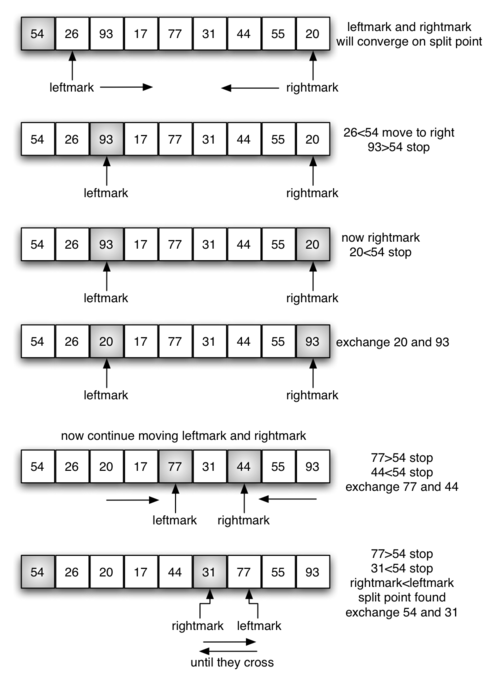
\includegraphics{quick-sort-example.png}

\subsubsection{Complessitá}
Nel caso ottimo, il pivot ha esattamente metá degli elementi maggiori e metá minori. L'algoritmo é analogo al merge sort, quindi $$T(n) = 2T(\frac{n}{2}) + \Theta(n) = \Theta(nlogn)$$
Nel caso pessimo, l'array é (paradossalmente) giá ordinato. Ogni elemento ha tutti gli elementi a destra maggiori: ad ogni ciclo si decrementa $j$ (ci si sposta dal fondo verso l'inizio) fino a raggiungere $i$, siccome il primo elemento di ogni ciclo é giá nella posizione corretta. $$T(n) = T(n-1) + \Theta(n) = \Theta(n^2)$$
Nel caso medio, considerando il caso in cui il pivot abbia $\frac{1}{10}$ degli elementi piú piccoli e $\frac{9}{10}$ piú grandi, si puó costruire un albero di decisione (qui considera il caso di $\frac{1}{4}$ e $\frac{3}{4}$ ma sono analoghi):

\begin{figure}
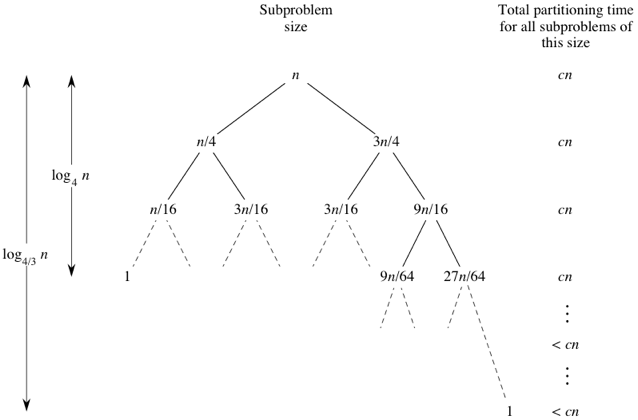
\includegraphics[scale=0.5]{quick-sort.png}
\caption{Fonte: Khan Academy}
\end{figure}

Fino a quando ci sono tutti i rami, si paga $log_{10}n$ volte $n$ ($\frac{1}{10}n+\frac{9}{10}n, \frac{1}{100}n+\frac{9}{100}n+\frac{9}{100}n+\frac{81}{100}n, \dots$); una volta che una parte dei rami termina, si paga $\displaystyle log_{\frac{10}{9}}n$ volte una quantitá $< n$, quindi la complessitá totale é $\Theta(nlogn)$.

\end{document}